\documentclass[12pt,a4paper]{article}
\usepackage[utf8]{inputenc}
\usepackage{fullpage}
\usepackage{url}
\usepackage{hyperref}   
\usepackage{tikz}
\usepackage[margin=1cm]{caption}
\usepackage{anyfontsize}
\usetikzlibrary{matrix,arrows.meta,fit,positioning,shapes}

\usepackage{parskip}
\setlength{\parindent}{0pt}
% \setlength{\parskip}{\baselineskip}


\title{\fontsize{42}\Huge\sc swarm\\\ \\
\vspace{1.5cm}
\Large storage and communication infrastructure\\ for a self-sovereign digital society}

\author{Authored by the Swarm team}
\date{v1.0 of \today}

\begin{document}
\maketitle
\vspace{.5cm}
\begin{center}

\includegraphics[width=0.2\textwidth]{fig/logo.pdf}
\end{center}
\vspace{1.5cm}
\noindent
%\section{Introduction}
\renewcommand{\abstractname}{}
\begin{abstract}
\noindent
Swarm is a peer-to-peer network of nodes that collectively provide a decentralised storage and communication service. This system is economically self-sustaining due to a built-in incentive system which is enforced through smart contracts on the Ethereum blockchain and powered by the BZZ token.

\noindent
In this paper, we first introduce Swarm's network layer that implements a distributed archive of fixed sized data units. Next we describe high level functionality provided by the API which renders Swarm a viable development stack and deployment environment for the decentralised web. 
    
\end{abstract}
\newpage
\tableofcontents
\section*{}
\listoffigures
\newpage
\section{Introduction}

Swarm’s mission is to shape the future towards a self-sovereign global society and permissionless open markets by providing scalable base-layer infrastructure for the decentralised internet. Swarm’s vision is to extend the blockchain with peer-to-peer storage and communication to realise the world computer that can serve as an operating system and deployment environment for decentralised applications.  

Swarm provides continuity of service and resilience against network outages or targeted denial of service attacks. As a platform for permissionless publication, Swarm fosters freedom of information. With its exceptional privacy features like anonymous browsing, deniable storage, untraceable messaging and file representation formats that leak no metadata, Swarm responds to the growing demand for security on the web. 

Built-in incentives seek to optimise the allocation of bandwidth and storage resources and render Swarm economically self-sustaining. Swarm nodes track their relative bandwidth contribution on each peer connection, and excess debt due to unequal consumption can be settled in BZZ. Publishers in Swarm must spend BZZ to purchase the right to write data to Swarm and prepay some rent for long term storage.

An example of modular design, 
Swarm consists of clearly separable layers (see figure \ref{fig:Swarm-layered-design}).
Technically, (2) and (3) constitute the core of Swarm and are discussed in the following two sections of this paper.

\begin{figure}[htbp]
  \centering
    
\includegraphics[width=\textwidth]{fig2/swarm-layered-design.pdf}
  \caption[Swarm's layered design]{Swarm's layered design}
\label{fig:Swarm-layered-design}
\end{figure}    


\section{DISC: Distributed Immutable Store of Chunks}
The DISC (\/\emph{Distributed Immutable Store of Chunks}) is the underlying storage model of Swarm. It consists of nodes that collaborate in storing and serving data in such a way that, while individual nodes are assumed to pursue strategies that maximise their operator's profit, the behaviour of the network as a whole attains the following emergent properties:

\begin{itemize}
    \item 
Privacy-preserving and permissionless upload and download
\item
Robust defences against blocking or changing access to content once published
\item
Auto-scaling with increased demand
\item 
Integrity protected content
\item 
Eventually forgetting content that is no longer relevant to preserve
\end{itemize}

Participating in the DISC as a node operator and being rewarded for doing so is possible for anyone with spare storage and bandwidth capacity. When the operator installs and runs the Swarm client software, a new node is created and becomes part of the network, essentially taking care of one sector of Swarm's global hard-drive.

In what follows, we define the DISC and explain how it gives rise to the properties above.

\subsection{Connectivity, topology, and routing}

The initial responsibility of the DISC is to build and maintain a network of nodes in such a way that all nodes can send messages between each other. This exchanging of messages happens via long-lasting and secure communication channels between nodes using peer-to-peer network protocols (libp2p%
\footnote{\url{https://libp2p.io/}}) 
. Swarm expects nodes to build up \emph{Kademlia}%
\footnote{\url{https://link.springer.com/chapter/10.1007\%2F3-540-45748-8_5}} connectivity:
connect to a specific subset of other nodes in such a way that nodes' local decisions about where  to forward result in globally optimal routing of messages.% travelling between nodes in the network.


Kademlia assumes that each node is assigned a \emph{Swarm address} which is distinct from their network address. By counting the number of prefix bits, two Swarm addresses have in common, we can define their degree of \emph{proximity}. Nodes that are closest to each other form a fully connected \emph{neighbourhood}. Additionally, each node connects to a number of peers from each discreet proximity class (see figure \ref{fig:swarm-kademlia}).


\begin{figure}[!ht]
   \centering
   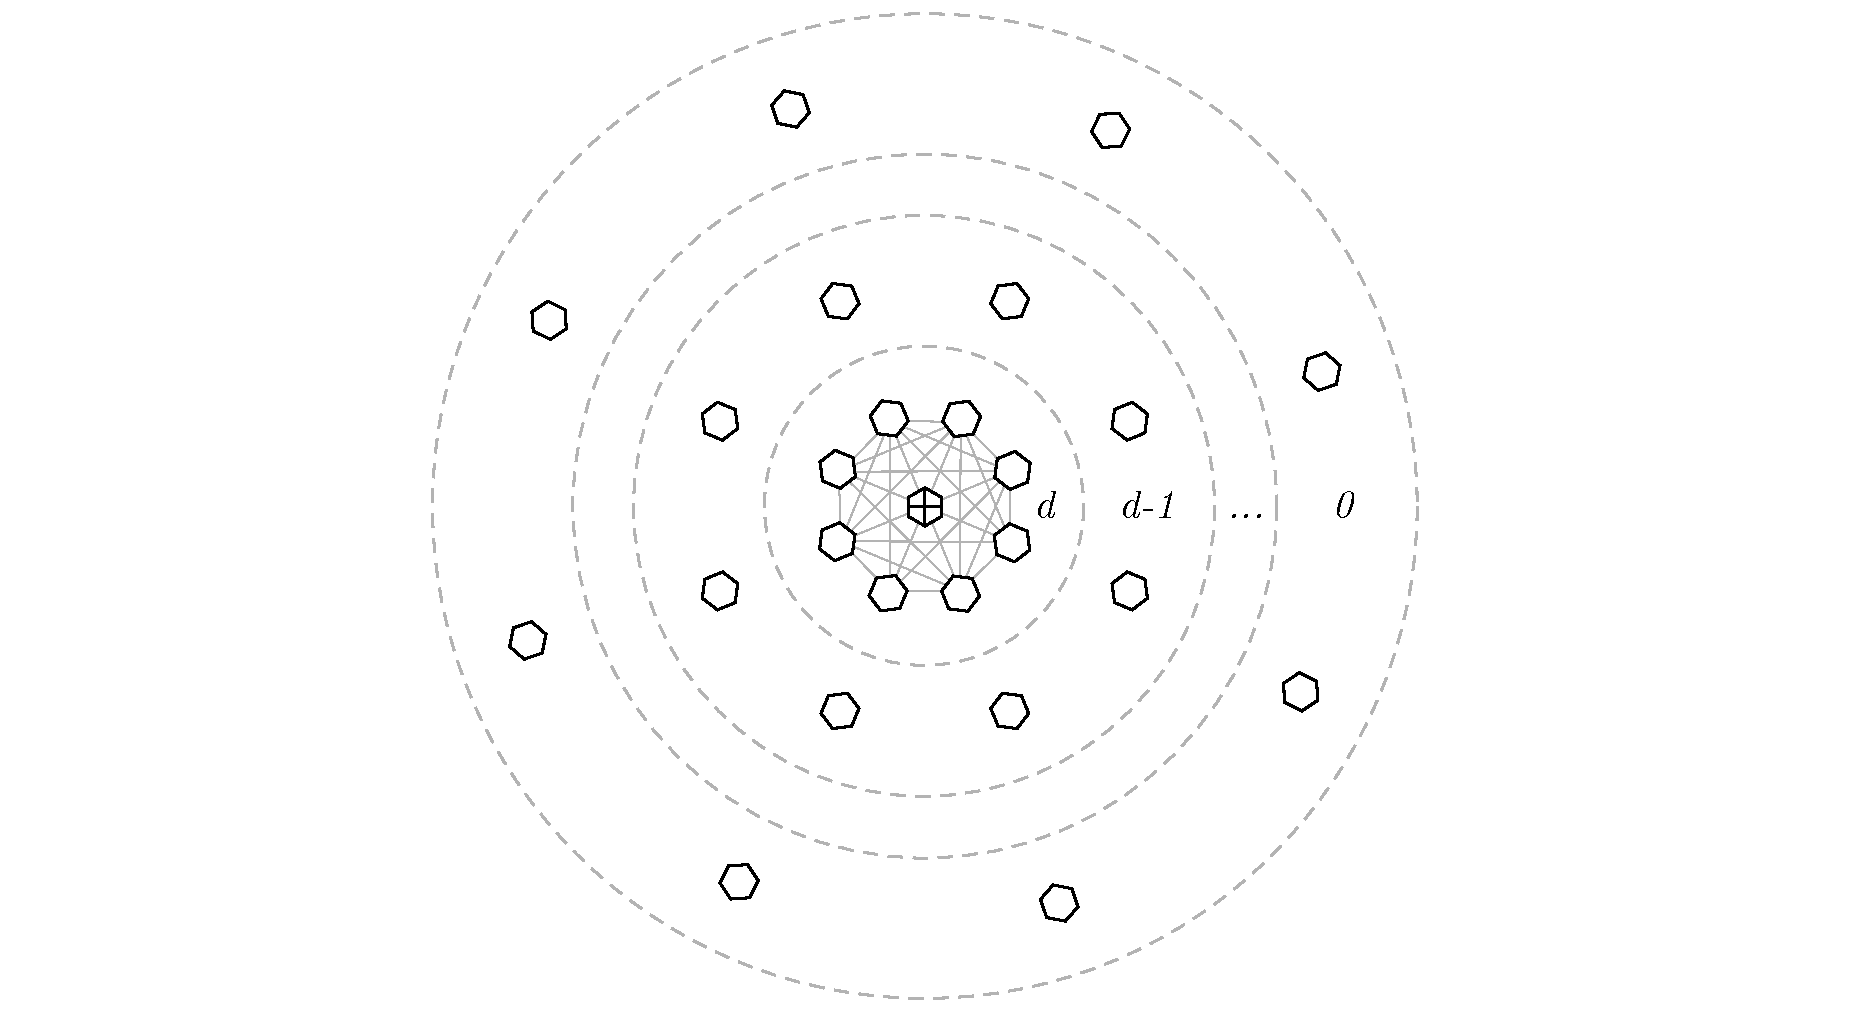
\includegraphics[width=\textwidth]{fig2/swarm-kademlia.pdf}
   \caption[Kademlia connectivity]{Kademlia connectivity. The fully connected neighbourhood containing minimum 8 nodes is defined by proximity order $d$, The node is also connected to  at least 8 balanced peers in each shallower proximity bucket $d-1, \ldots, 0$. }
   \label{fig:swarm-kademlia}
\end{figure}

The resultant topology guarantees that relaying moves a message at least one step closer to its intended destination on each hop (see figure \ref{fig:request-response}). This technique enables messages to be routed between any two nodes, even if they do not maintain a direct connection. The number of hops required to deliver messages has an upper bound that is logarithmic in the total number of nodes, thus ensuring that any two nodes will always be able to reach each other, even in an extremely large network.


\begin{figure}[!ht]
   \centering
   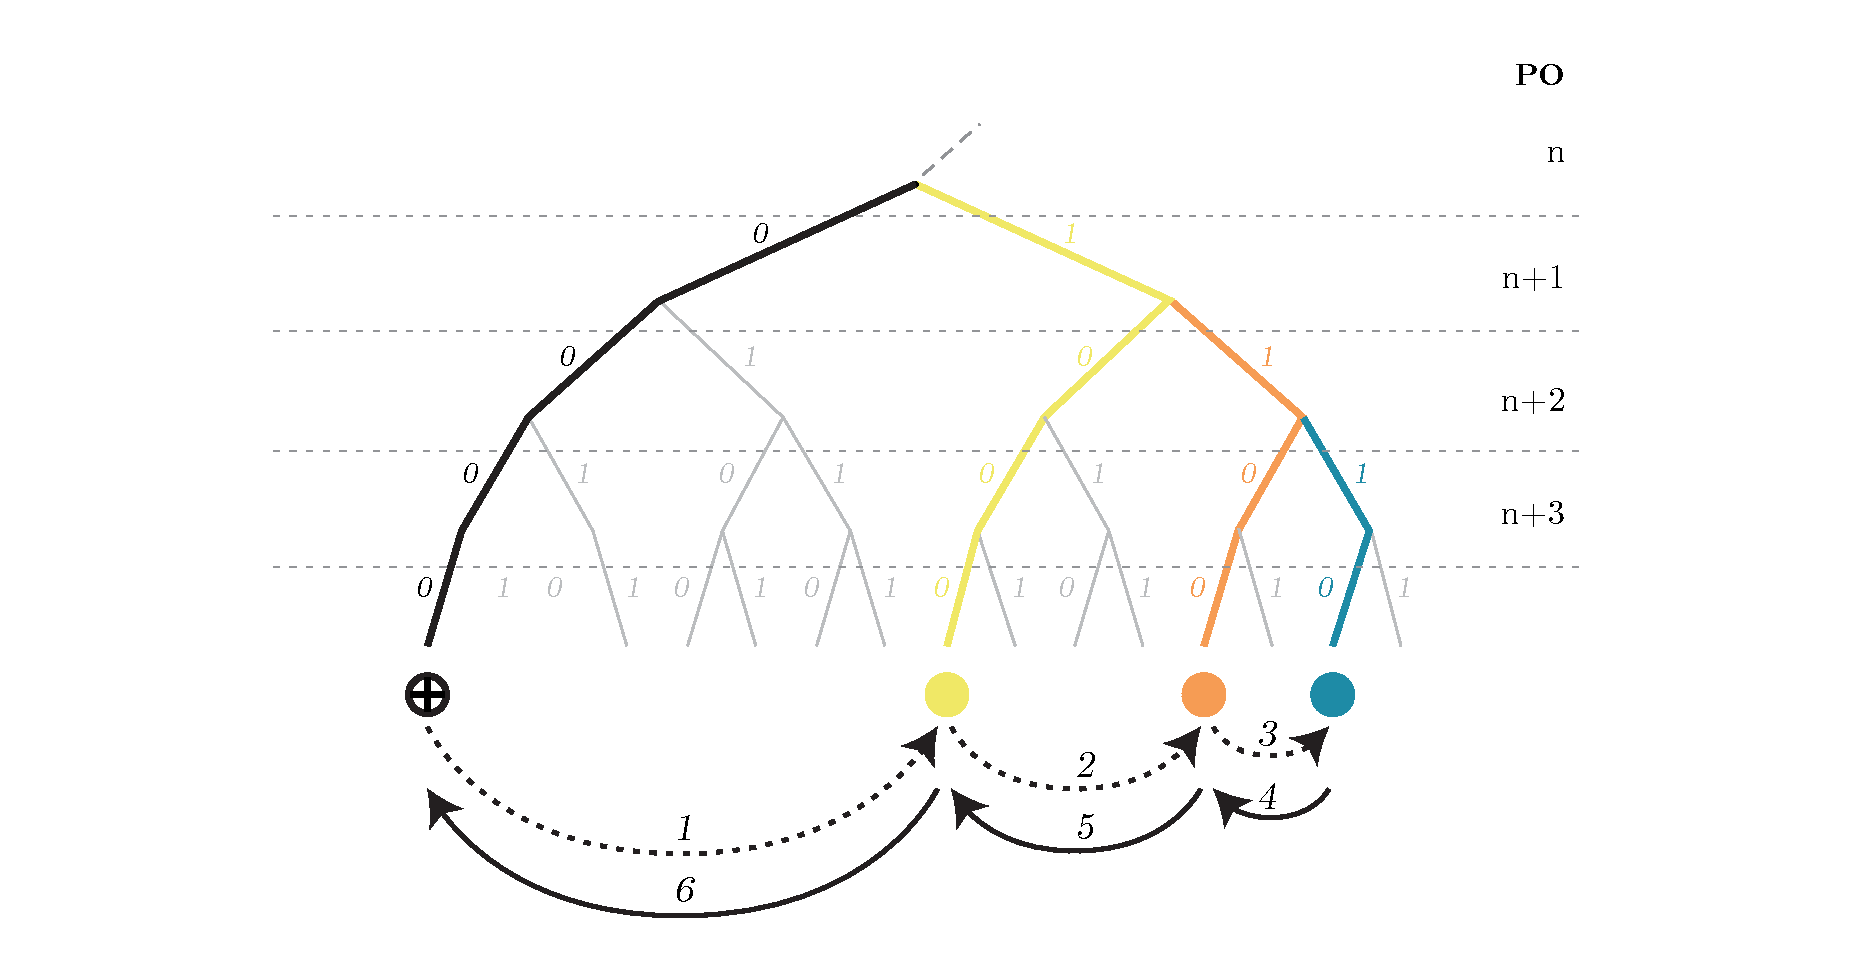
\includegraphics[width=\textwidth]{fig2/request-response-forwarding.pdf}
   \caption[Request-response round-trips in forwarding Kademlia]{Request--response round-trips in forwarding Kademlia. Here a node with overlay address $...0000...$ is sending a request to target $....1111...$ to which the closest online node is $...1110...$ The leading ellipsis represents the prefix shared by the requestor and target which has a length of $n$ bits, the trailing ellipsis represents part of the address that is not relevant for routing as at that depth nodes are already unique. The requestor forwards a message to the connected peer they know that is nearest to the destination (yellow). The recipient peer does the same. Applying this strategy recursively relays the message via a chain of peers (yellow, orange, blue) each at least one PO closer to the destination. Relaying nodes on the way remember the peer a request came from so that when the response arrives, they can \emph{backward} it (i.e.\ pass it back) along the same route.}
   \label{fig:request-response}
\end{figure}

\subsection{Chunks and storage}

The canonical unit of storage in Swarm is called a \emph{chunk}. A chunk consists of at most 4 kilobytes of data and has an address. Since a chunk’s address is taken from the same address space as a node’s address, it is possible to compute their proximity. Swarm’s storage scheme declares that each chunk is stored by the nodes with an address that is close to that of the chunk itself. 


To facilitate the confidentiality of data, chunks can be padded to 4 kilobytes and then encrypted, making them indistinguishable from random data for anyone without the decryption key. Even for unencrypted chunks, there is no easy way for node operators to figure out which content a chunk forms part of. Since Swarm nodes do not get to choose which chunks they store, encryption, ambiguity of context and lack of leaked metadata all provide them protection against liability for the content they host.

To insert a chunk into the swarm, nodes relay the chunk via the push-sync protocol until it arrives at the neighbourhood it belongs to. A statement confirming the storage of the chunk is then passed back along the same route. In order to retrieve a chunk, a request with a chunk address is routed towards the relevant neighbourhood using the retrieval protocol. If any node on the way has the corresponding chunk in their local storage, it is sent back as a response.

\begin{figure}[htbp]
  \centering
    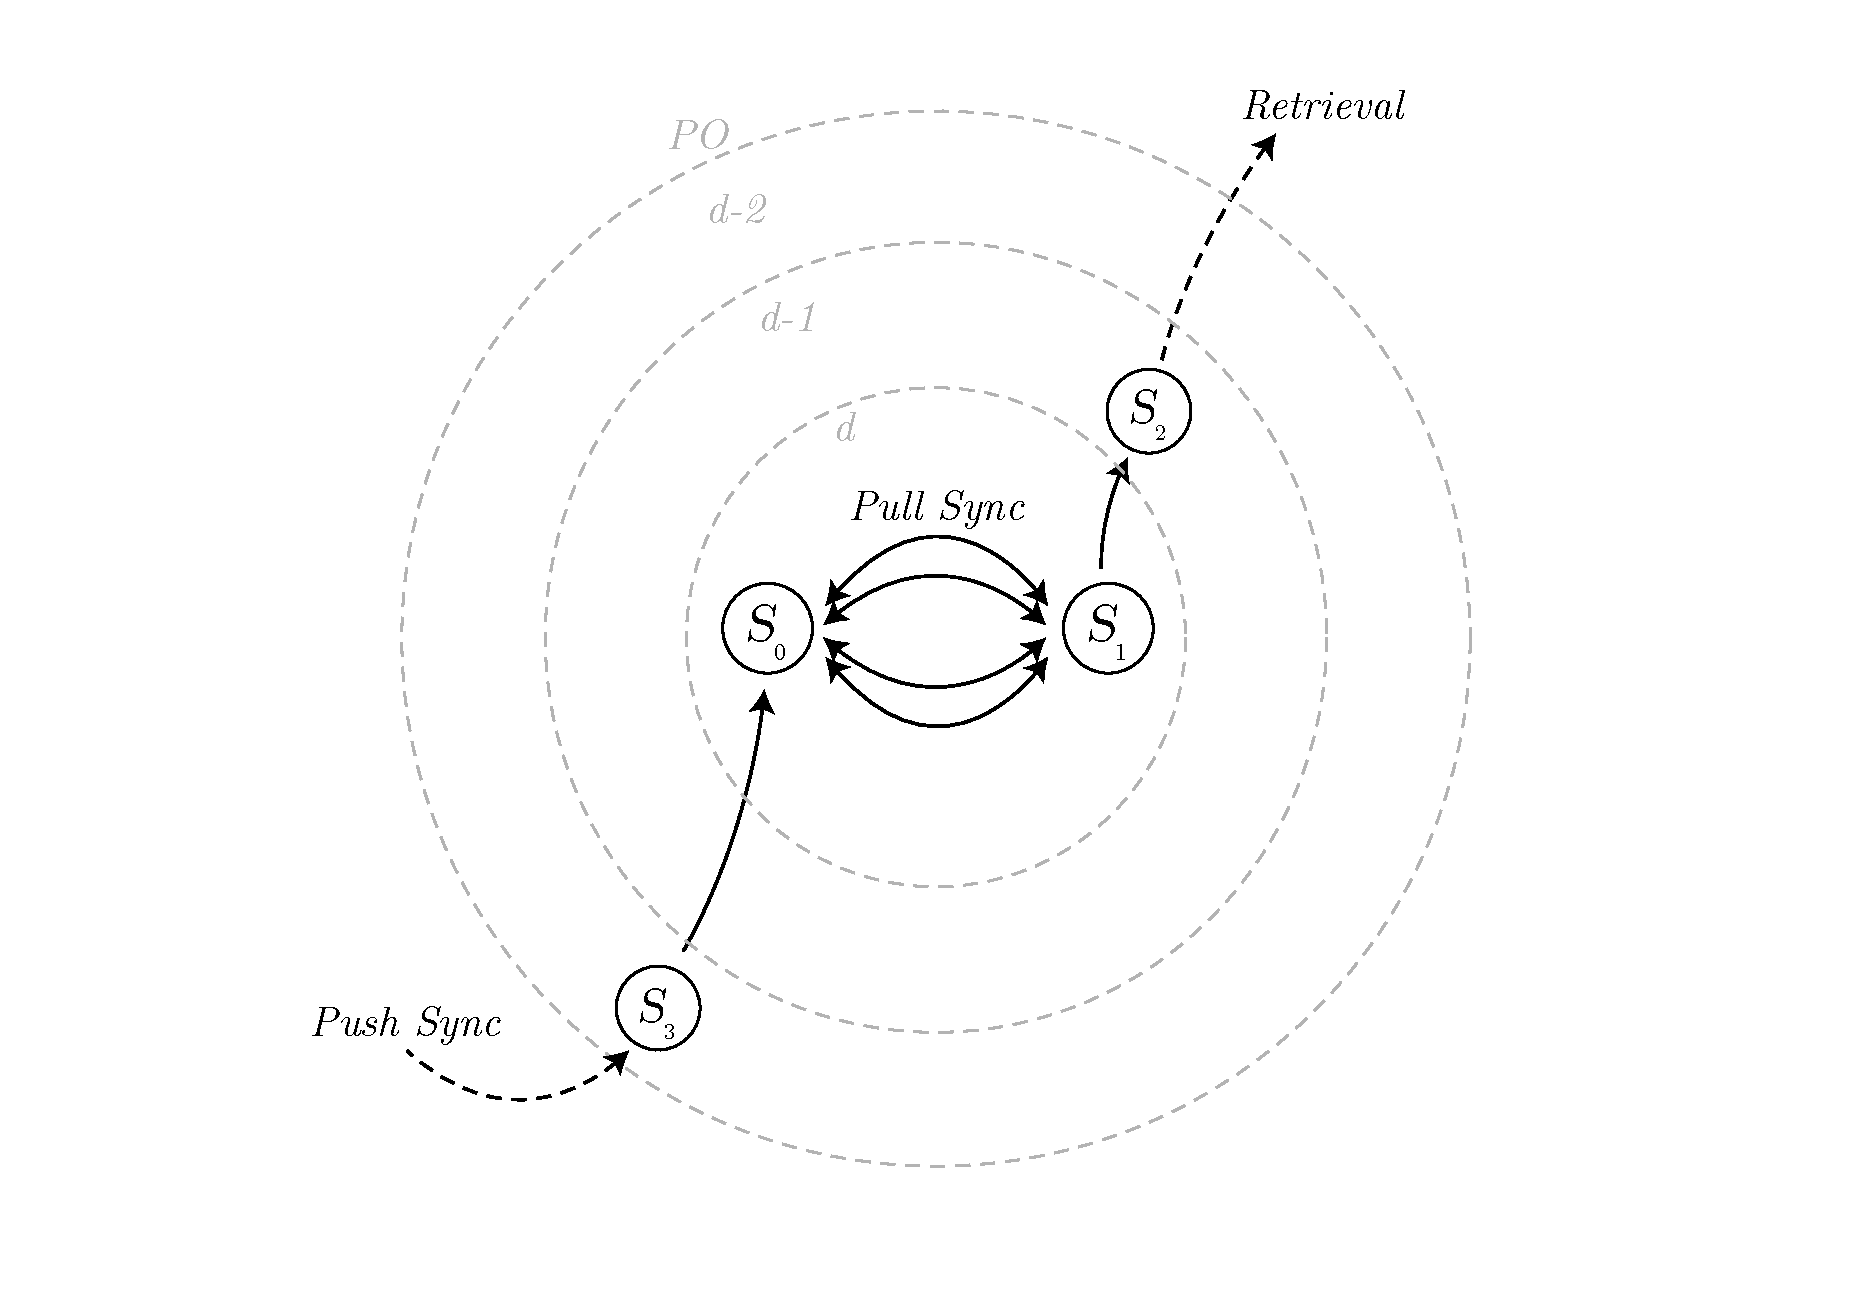
\includegraphics[width=\textwidth]{fig2/pull-push-retrieve.pdf}
  \caption[Push, Pull and Retrieve Protocols]{Push, Pull and Retrieve Protocols}
\label{fig:push-pull-retrieve}
\end{figure}

Nodes continuously synchronise their chunk storage using the pull-sync protocol. This guarantees that all chunks that belong to their neighbourhood are redundantly stored by each neighbour. This redundancy adds resilience, sustaining a chunk's availability in the case that some of the nodes in the neighbourhood are unreachable. The synchronisation protocol also ensures that the neighbourhoods' storage is consistent as nodes go offline and new nodes join the network. 

\subsection{Forwarding, privacy, and caching}

In the swarm, routing a message is achieved by recursively forwarding it ever closer to its destination, and then passing back a response along the same route. This routing algorithm enables two important properties:

\begin{itemize}
    \item Ambiguity of who has initiated the request.
    \item Automatic scaling with increased demand.
\end{itemize}

A message by a node initiating the request is in every way identical to a message from a node simply forwarding a request. This ambiguity enables the originator of the request to preserve their privacy, thus facilitating permissionless publishing and private browsing.

Automatic scaling of distribution is enabled because nodes who participate in routing retrieval requests may choose to store the chunks they have forwarded. Economic motivation for such \emph{opportunistic caching} is provided by the bandwidth incentives discussed next.

\subsection{Swarm Accounting Protocol}

The \emph{Swarm Accounting Protocol} (SWAP) ensures that node operators collaborate in routing messages, while protecting the network against frivolous use of bandwidth.

As nodes relay requests and responses, they keep track of their relative consumption of bandwidth with each of their peers. Within bounds peers engage in a service-for-service exchange.
However, once a limit is reached, the party in debt can either wait until their liabilities are amortised over time, or can pay by sending cheques that cash out in BZZ on the blockchain (see figure \ref{fig:swap}).


\begin{figure}[!ht]
  \centering
    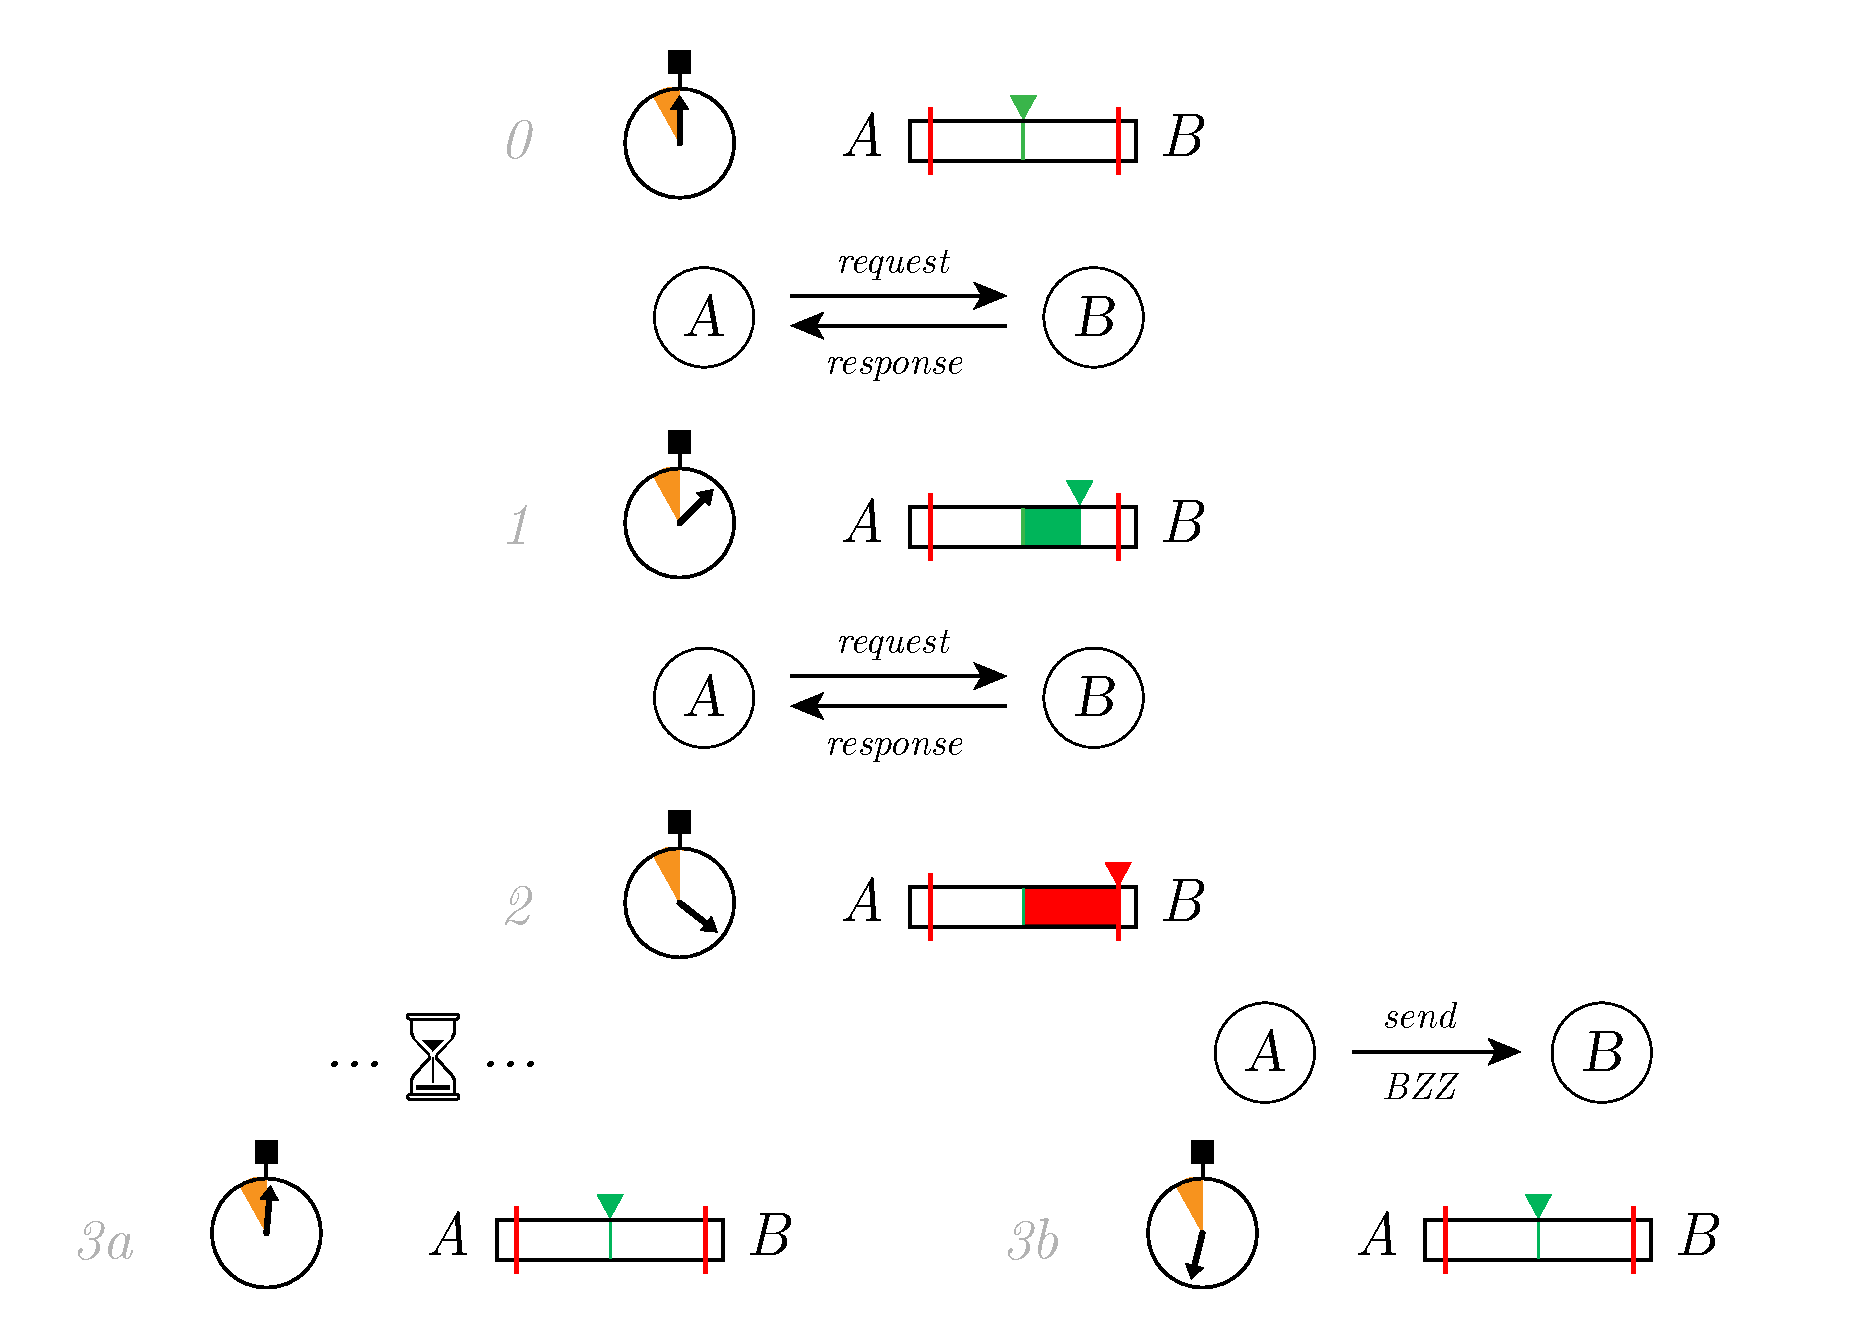
\includegraphics[width=.9\textwidth]{fig2/SWAP5.pdf}
  \caption[Swarm Accounting Protocol]{Swarm Accounting Protocol. This figure illustrates how peers keep track of each other's bandwidth contribution. Starting from zero balance on both sides at step 0 is followed by a period of message exchange and leads through step 1, to step $n$, all the way where the debt on one side reaches a threshold. The debt can be reduced over time or the peer in credit gets compensation.}
\label{fig:swap}
\end{figure}

This protocol ensures that Swarm is free to use for those who are downloading or uploading a small amount of content or are willing to wait until they have earned credit by providing reciprocal services on each peer connection. At the same time, a snappy experience when uploading or downloading higher volumes is enabled for those who wish to pay.

Nodes are financially motivated to help each in relaying messages, because each node that successfully routes a request closer to the destination earns BZZ when the request was successfully served. If that node is not storing the data itself, it pays a small amount of money to request chunks from an even closer node. By doing such trades, nodes earn a little profit when serving a request. This implies that nodes are motivated to cache chunks as, after purchasing the chunk once from a closer node, any subsequent requests for the same chunk will earn pure profit.

\subsection{Capacity shortage and garbage collection}

As new content gets added to Swarm, sooner or later, the finite storage capacity of each node will be used up. At this point nodes need a strategy to decide which chunks should be removed to make way for new chunks. 

Each Swarm node’s local storage has two subsystems, the \emph{reserve} and the \emph{cache}.


The reserve is a fixed size of storage space dedicated to store chunks that belong to the node's neighbourhood. Whether or not a chunk is retained in the reserve is determined by the \emph{postage stamp} attached to it. A contract on the blockchain allows advance purchase of a \emph{postage batch} for BZZ tokens. A batch entitles the owner to issue a limited number of stamps. These stamps then serve as a fiduciary signal indicating how much it is worth for a user to persist the associated content in Swarm. 
By using this value to prioritise which chunks to remove from the reserve first, storer nodes maximise the utility of the DISC (see figure \ref{fig:postage-stamps}). 
The value of a postage stamp decreases over time as if storage rent was regularly deducted from the batch balance; once the value of a stamp is no longer sufficient, the associated chunk is evicted from the reserve and put into the cache. 

\begin{figure}[!ht]
  \centering
    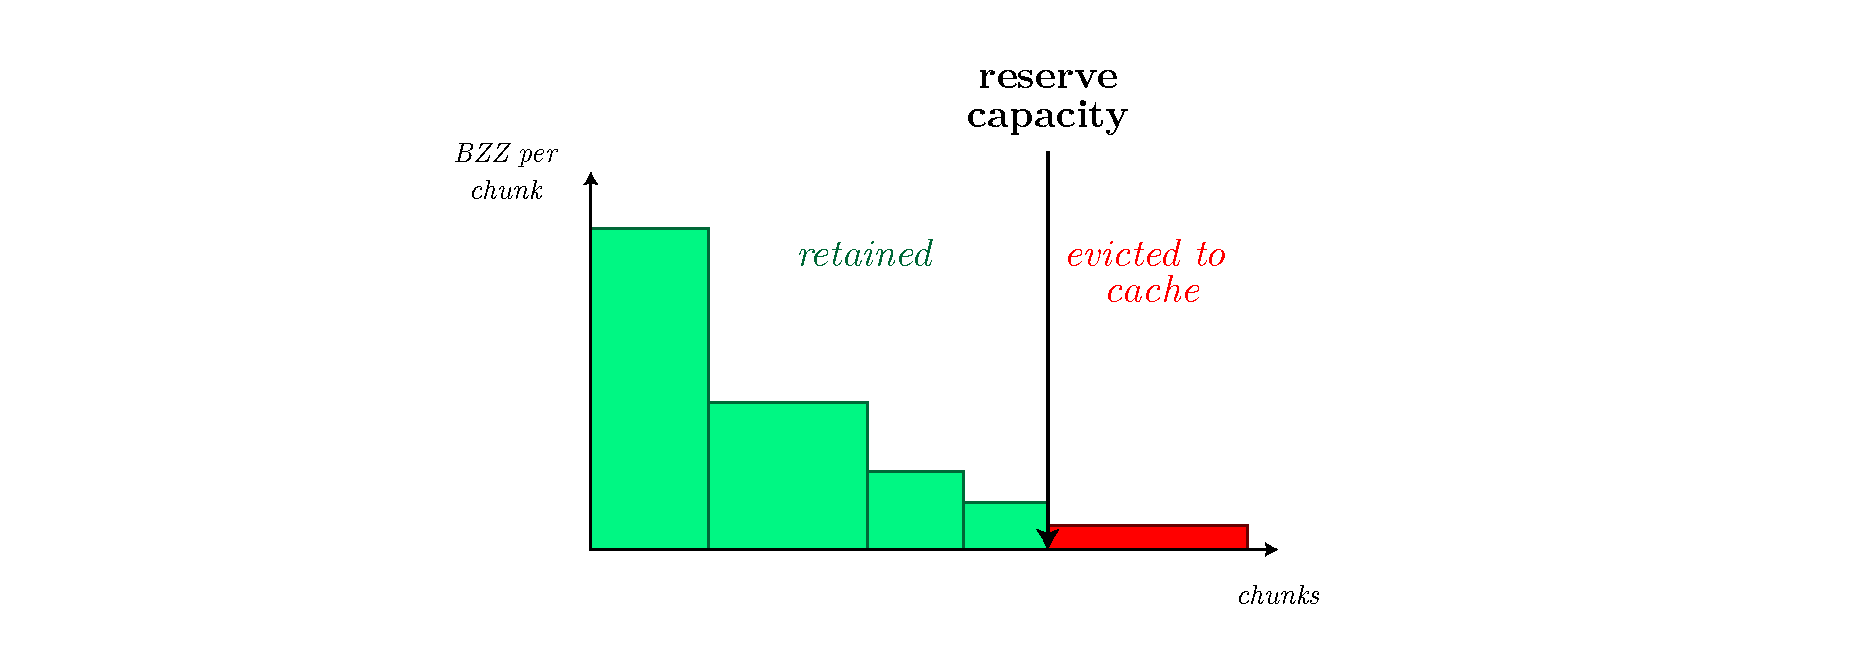
\includegraphics[width=\textwidth]{fig2/reserve-capacity-2.pdf}
  \caption[Postage Stamp Priority]{Postage Stamp Priority}
\label{fig:postage-stamps}
\end{figure}    


The role of the cache is to retain chunks not protected by the reserve either due to insufficient batch value or because they are too far from the node address. The cache is pruned regularly when capacity is reached by removing the chunks that were requested the longest time ago. As the recency of the last request is a reasonable predictor of popularity, chunks with more SWAP income will be preferentially retained. Combined with opportunistic caching, this garbage collection strategy maximises the operator's profit from the bandwidth incentives, while on the network level, implements automatic scaling of popular content.

\subsection{Chunk types}

Previously, we have defined chunks as the canonical unit of data in the DISC. There are two fundamental chunk types: \emph{content-addressed chunks} and \emph{single-owner chunks}. 

The address of content-addressed chunks is based on the hash digest of its data (see figure \ref{fig:content-addressed-chunk}). Using a hash as the chunk address makes it possible to verify the integrity of chunk data. Swarm uses the \emph{BMT hash} function based on a binary Merkle tree over small segments of the chunk data. 

\begin{figure}[!ht]
   \centering
   
\includegraphics[width=\textwidth]{fig2/content-addressed-chunk-3.pdf}
   \caption[Content addressed chunk]{A content addressed chunk has an at most 4KB payload. The address is calculated as the hash of the span and the Binary Merkle Tree hash of the payload.}
   \label{fig:content-addressed-chunk}
\end{figure}



The address of a single-owner chunk is calculated as the hash of the owner’s address and an identifier. The integrity of single-owner chunk data is warranted by the cryptographic signature of the owner attesting to the association of arbitrary chunk data with the identifier  (see figure \ref{fig:single-owner-chunks}). In other words, each identity owns part of Swarm's address space within which they are free to assign content to an address.

\begin{figure}[!ht]
   \centering
   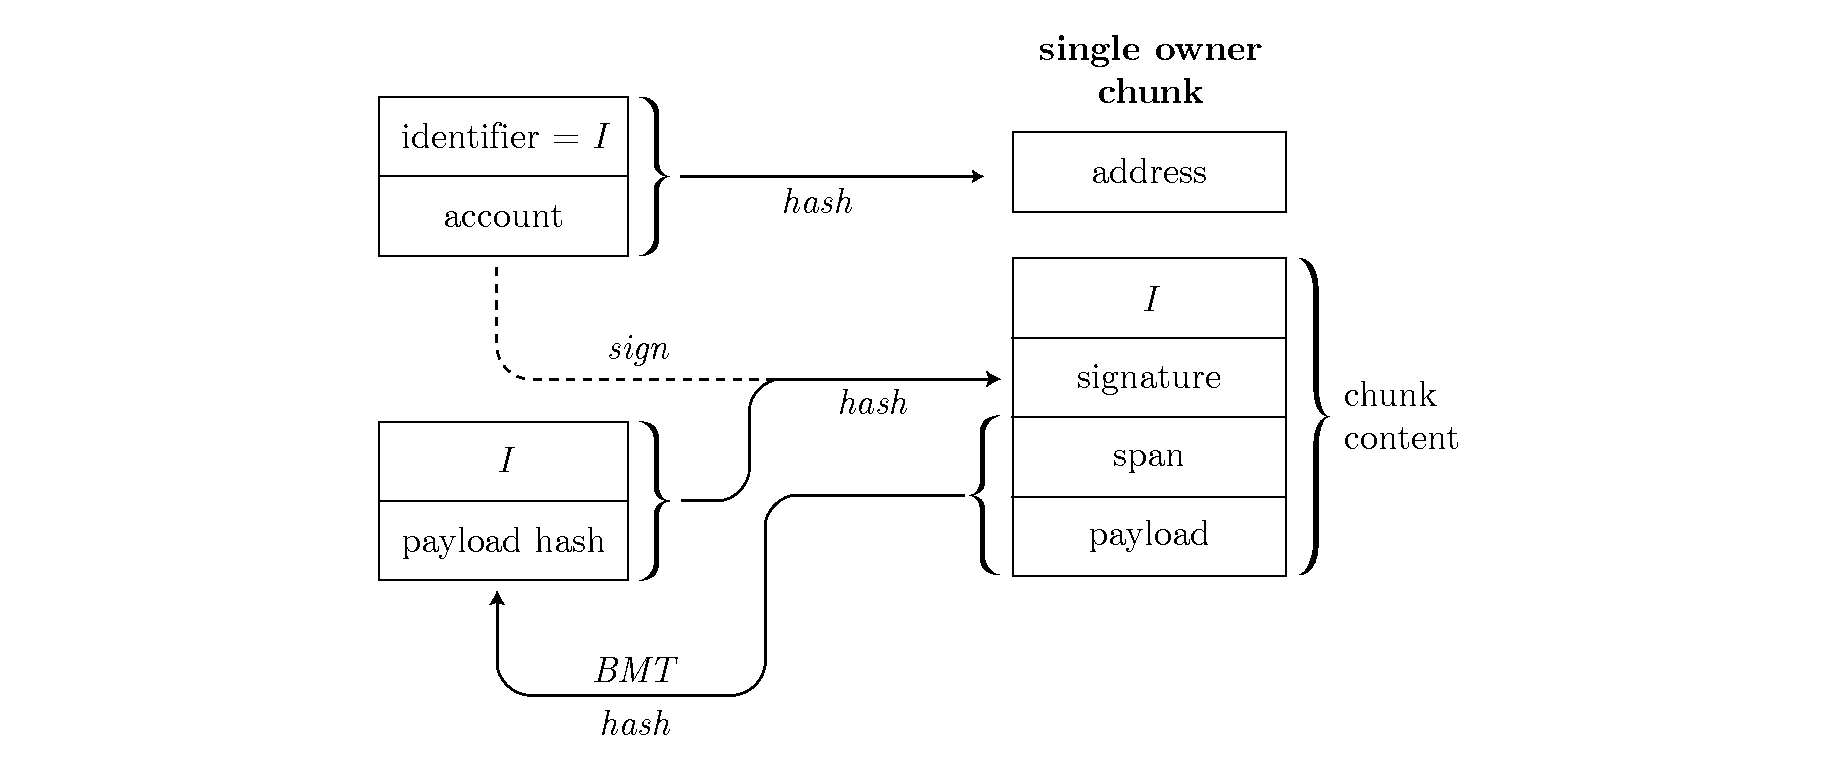
\includegraphics[width=\textwidth]{fig2/single-owner-chunk.pdf}
   \caption[Single-owner chunk]{Single-owner chunk. The chunk content is composed of headers followed by an at most 4KB payload. The last header field is the 8 byte span prepended just like in content addressed chunks. The first two header fields provide single owner attestation of integrity: an identifier and a signature signing off on the identifier and the BMT hash of span and payload. The address is the hash of the id and the signer account.}
   \label{fig:single-owner-chunks}
\end{figure}


\section{Functionality of the Swarm API}

Beyond chunks, Swarm also exposes APIs for dealing with higher-level concepts such as files, hierarchical collections of files with various metadata, and even inter-node messaging. The APIs seek to mirror those already in use on the web. Further novel constructs and data structures can be mapped upon or alongside these higher layer patterns, giving rise to a rich and diverse range of possibilities for anyone wishing to benefit from the core offerings of privacy and decentralisation afforded by the DISC.

\subsection{Files and collections}



Data which is larger than the 4 kilobytes allowed in a single chunk is split into many. A set of chunks belonging together are represented by a swarm hash-tree which encodes the way in which a file was split into chunks during its upload. This tree consists of a set of leaf node chunks, containing the data itself, which are referenced by one or several layers of intermediate chunks, each containing references to their children chunks (see figure \ref{fig:Swarm-hash}).

\begin{figure}[!ht]
\centering
\resizebox{1\textwidth}{!}{
    \input{fig/Swarm-hash.tex}
}
\caption[Swarm hash]{Swarm hash: data input is segmented to 4-kilobyte chunks (gray), that are BMT hashed. Their hashes are packaged into intermediate chunks starting on level $0$, all the way until a single chunk remains on level $n$. }
\label{fig:Swarm-hash}
\end{figure}

The content address of the whole file is then determined by the hash digest of the root chunk, i.e. the Merkle root of the hash tree spanning the entire file. In this way, a file’s address becomes its checksum, enabling verification of the integrity of content. Representing files as a balanced Merkle tree of chunks also provides efficient random access in files and, as a result, range queries can be served efficiently. 

To represent collections, Swarm uses \emph{manifests}. A manifest encodes a generic string-reference mapping allowing it to model a directory tree, a key--value store or a routing table. These respectively enable Swarm to implement a file system, serve as a database, and even provide virtual hosting for websites and dapps.



Manifests offer URL-based addressing if we interpret the host part of the URL as referencing a manifest, while the URL path is used as the key looked up in the map that the manifest represents only to arrive at a file reference. 

Manifests encode the map they represent in the form of a compacted Merkle trie, with chunks serialising the nodes of the trie (see figure \ref{fig:manifest-structure}). When a path is looked up, we only need to retrieve the chunks that correspond to nodes along the branches we traverse. This ensures efficient lookup of files/records with latency and bandwidth overhead that is logarithmic in the size of the collection. 


\begin{figure}[!ht]
\centering
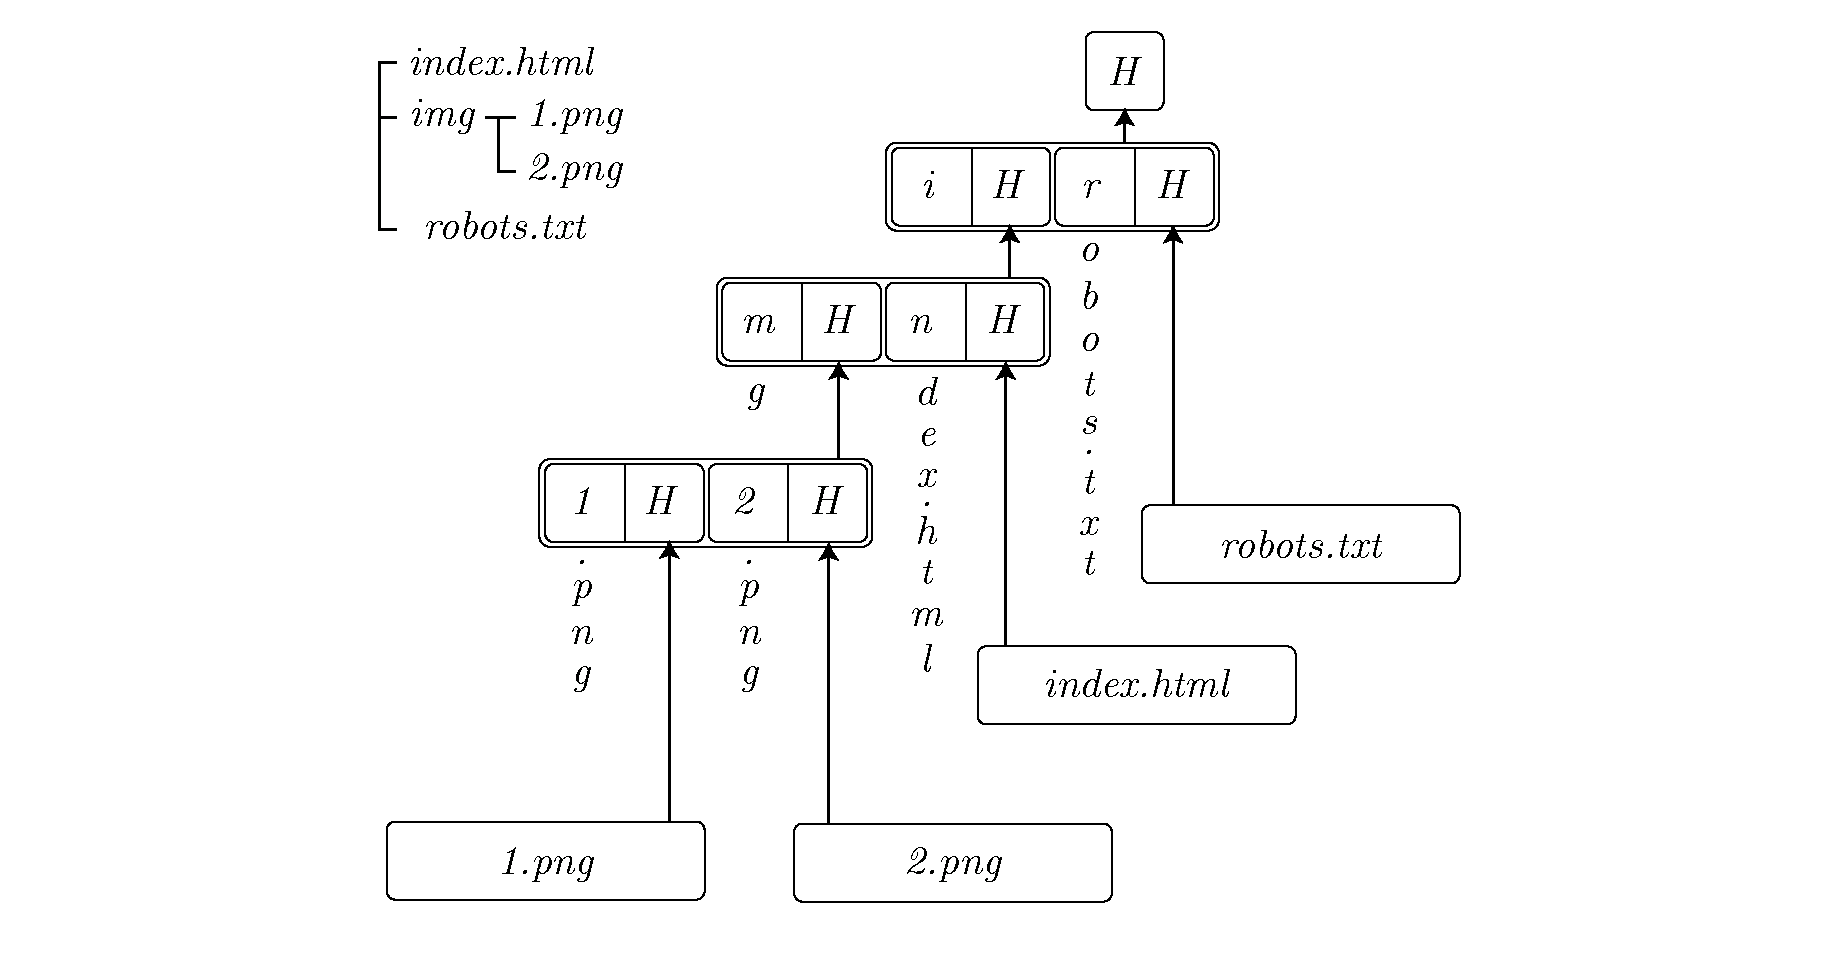
\includegraphics[width=\textwidth]{fig2/manifest-structure.pdf}
\caption[Manifests]{Manifest chunks represent nodes of a compacted trie: they enlist continuations indexed by the next byte of the key. The continuation specifies the reference to a file with the remainder of the key or, if there are still several continuations, the reference to the trie node corresponding to the next fork on the path together with the longest shared prefix.}
\label{fig:manifest-structure}
\end{figure}


Child node references in intermediate chunks of the hash tree for files, and manifest trie nodes for collections, positionally align with segments of the BMT hash. As a consequence, Swarm supports compact proofs that a particular data segment is part of a file at a given URL at a given offset, which is the basis for publicly provable database indexes and trustless aggregation.


\subsection{Tracking updates: feeds and domain resolution}

A feed is an example of a single-owner chunk that allows the impression of a mutable resource. Feeds are able to represent, amongst other things, versioned revisions of a mutable resource, sequential updates to a topic or consecutive messages posted by one party in a communication channel. 

Feeds work by defining the identifier of a single-owner chunk as derived from a topic and an index. When the publisher and the content consumer agree on how and when the index is updated, a specific reference to a feed update can be constructed and looked up.

Analogous to how DNS resolves domains to the IP address of host servers, Swarm supports human-readable domain names (e.g. swarm.eth) by resolving them to references using the Ethereum Name Service, a set of smart contracts on the blockchain. 

The reference registered in ENS may be updated whenever the web application or website it represents got a new swarm reference because of an update. Optionally, when  a domain name references a \emph{feed}, users can benefit from human readable domain names, while also being able to update their content without interacting with the blockchain for each change and paying the associated transaction cost.

\subsection{Messaging}

PSS (Postal Service on Swarm) is a protocol for direct node-to-node messaging in Swarm. It is implemented by encrypting a message for the intended recipient, and wrapping it with a topic in a content addressed chunk. Since the chunk is crafted in such a way that its content address falls into the recipient’s neighbourhood, delivery is naturally taken care of by the push-sync protocol. 

Furthermore, for any third party, the message is indistinguishable from a random encrypted chunk, hence the name ‘Trojan’ chunk. A node expecting to receive PSS messages would attempt to decrypt and unwrap all chunks arriving in its neighbourhood. After successfully decrypting and unwrapping a Trojan chunk as a rightful recipient, the client node can dispatch the message plaintext to applications that have subscribed to that topic using the PSS API.

PSS also offers asynchronous delivery, because chunks are persisted and eventually synced to all neighbourhood nodes even if they come online at a later time. 

As PSS allows users to receive messages from hitherto not known identities, it is an ideal communication primitive for sending anonymous messages to a public identity, e.g., registrations, or initial contact to start a thread by setting up a secure communication channel using feeds. Since PSS does not require action (e.g., polling) from the recipient, it serves as the recommended primitive for push notifications. 

\subsection{Pinning and Recovery}

The DISC eventually forgets content that is rarely accessed and not paid for. By \emph{pinning} chunks, nodes can ensure they will preserve specific content locally. However, such local \emph{pinners} can participate in a reactive or proactive \emph{recovery} of content for the benefit of all users.

Reactive recovery involves a recovery protocol which, in the event of failed retrieval, notifies a pinner about a missing chunk by sending a recovery request using PSS. Pinners listen to recovery requests and respond by re-uploading the missing chunk that the downloader will then find upon retry. This fallback recovery feature also enables seeding original content directly from a publisher node, and resembles the primary mode of operation in some existing file-sharing solutions (BitTorrent, IPFS).

Conversely, proactive recovery, or \emph{data stewardship} is provided when pinners proactively check the availability of content in the network and reupload chunks when they are found to be missing.

\section{Conclusion}
Swarm was introduced as a peer-to-peer network of nodes that collectively provide a decentralised storage and communication service. Permissionless and private, Swarm caters for freedom of expression, data sovereignty and open markets on the web while maintaining security with integrity protection, censorship resistance and attack resilience. This paper has covered functionalities that are included in the initial mainnet launch using Bee 1.0,%
\footnote{\url{https://github.com/ethersphere/bee/}}
%


With this milestone, the journey has only just begun: join the swarm%
\footnote{\url{https://ethswarm.org}}
%
on its mission of empowerment through digital freedom.

For a more thorough exploration of Swarm, read \emph{The Book of Swarm}%
\footnote{\url{https://www.ethswarm.org/The-Book-of-Swarm.pdf}}
\end{document}